%% (Master) Thesis template
% Template version used: v1.4
%
% Largely adapted from Adrian Nievergelt's template for the ADPS
% (lecture notes) project.


%% We use the memoir class because it offers a many easy to use features.
\documentclass[11pt,a4paper,titlepage]{memoir}

%% Packages
%% ========

%% LaTeX Font encoding -- DO NOT CHANGE
\usepackage[OT1]{fontenc}

%% Babel provides support for languages.  'english' uses British
%% English hyphenation and text snippets like "Figure" and
%% "Theorem". Use the option 'ngerman' if your document is in German.
%% Use 'american' for American English.  Note that if you change this,
%% the next LaTeX run may show spurious errors.  Simply run it again.
%% If they persist, remove the .aux file and try again.
\usepackage[english]{babel}

%% Input encoding 'utf8'. In some cases you might need 'utf8x' for
%% extra symbols. Not all editors, especially on Windows, are UTF-8
%% capable, so you may want to use 'latin1' instead.
\usepackage[utf8]{inputenc}

%% This changes default fonts for both text and math mode to use Herman Zapfs
%% excellent Palatino font.  Do not change this.
\usepackage[sc]{mathpazo}

%% The AMS-LaTeX extensions for mathematical typesetting.  Do not
%% remove.
\usepackage{amsmath,amssymb,amsfonts,mathrsfs}

%% NTheorem is a reimplementation of the AMS Theorem package. This
%% will allow us to typeset theorems like examples, proofs and
%% similar.  Do not remove.
%% NOTE: Must be loaded AFTER amsmath, or the \qed placement will
%% break
\usepackage[amsmath,thmmarks]{ntheorem}

%% LaTeX' own graphics handling
\usepackage{graphicx}

%% We unfortunately need this for the Rules chapter.  Remove it
%% afterwards; or at least NEVER use its underlining features.
\usepackage{soul}

%% This allows you to add .pdf files. It is used to add the
%% declaration of originality.
\usepackage{pdfpages}

%% Some more packages that you may want to use.  Have a look at the
%% file, and consult the package docs for each.
%% See the TeXed file for more explanations

%% [OPT] Multi-rowed cells in tabulars
%\usepackage{multirow}

%% [REC] Intelligent cross reference package. This allows for nice
%% combined references that include the reference and a hint to where
%% to look for it.
\usepackage{varioref}

%% [OPT] Easily changeable quotes with \enquote{Text}
%\usepackage[german=swiss]{csquotes}

%% [REC] Format dates and time depending on locale
\usepackage{datetime}

%% [OPT] Provides a \cancel{} command to stroke through mathematics.
%\usepackage{cancel}

%% [NEED] This allows for additional typesetting tools in mathmode.
%% See its excellent documentation.
\usepackage{mathtools}

%% [ADV] Conditional commands
%\usepackage{ifthen}

%% [OPT] Manual large braces or other delimiters.
%\usepackage{bigdelim, bigstrut}

%% [REC] Alternate vector arrows. Use the command \vv{} to get scaled
%% vector arrows.
\usepackage[h]{esvect}

%% [NEED] Some extensions to tabulars and array environments.
\usepackage{array}

\usepackage{braket}

\usepackage{tikz}
\usetikzlibrary{positioning,trees}

%% [OPT] Postscript support via pstricks graphics package. Very
%% diverse applications.
%\usepackage{pstricks,pst-all}

%% [?] This seems to allow us to define some additional counters.
%\usepackage{etex}

%% [ADV] XY-Pic to typeset some matrix-style graphics
%\usepackage[all]{xy}

%% [OPT] This is needed to generate an index at the end of the
%% document.
%\usepackage{makeidx}

%% [OPT] Fancy package for source code listings.  The template text
%% needs it for some LaTeX snippets; remove/adapt the \lstset when you
%% remove the template content.
\usepackage{listings}
%\lstset{language=TeX,basicstyle={\normalfont\ttfamily}}
\lstset{
language=C++,
basicstyle=\footnotesize\ttfamily,
keywordstyle=\bfseries\color{blue!60!black},
escapechar=@,
commentstyle=\itshape\color{purple!60!black},
numberstyle=\bfseries\color{red!60!black},
showstringspaces=false,
morekeywords={hsize_t},
breaklines=true,
breakatwhitespace=true,
literate=%
    {0}{{{\color{red}0}}}1
    {1}{{{\color{red}1}}}1
    {2}{{{\color{red}2}}}1
    {3}{{{\color{red}3}}}1
    {4}{{{\color{red}4}}}1
%    {5}{{{\color{red}5}}}1
    {6}{{{\color{red}6}}}1
    {7}{{{\color{red}7}}}1
    {8}{{{\color{red}8}}}1
    {9}{{{\color{red}9}}}1}

%% [REC] Fancy character protrusion.  Must be loaded after all fonts.
\usepackage[activate]{pdfcprot}

%% [REC] Nicer tables.  Read the excellent documentation.
\usepackage{booktabs}

\usepackage{amsmath}
\usepackage{amssymb}
\usepackage{amsfonts}
\usepackage{amsopn}
\usepackage{braket}
\usepackage{bbm}
\usepackage{dsfont}
% \usepackage{mathabx}


% Various new commands that ease typesetting math even further
% \newcommand{\assign}{\ensuremath{\coloneq}}
% \newcommand{\rassign}{\ensuremath{\eqcolon}}
\newcommand{\assign}{\ensuremath{:=}}
\newcommand{\rassign}{\ensuremath{=:}}
\newcommand{\seteq}{\ensuremath{\overset{!}{=}}}

\newcommand{\of}[1]{\ensuremath{\left( #1 \right)}}
\newcommand{\ofs}[1]{\ensuremath{\left( #1 \right)}}

%\newcommand{\norm}[1]{\ensuremath{\| #1 \|}}

\newcommand{\tmop}[1]{\ensuremath{\operatorname{#1}}}

\newcommand{\id}{\ensuremath{\mathds{1}}}
% \newcommand{\id}{\ensuremath{I}}

\newcommand{\kron}[1]{\ensuremath{\delta_{#1}}}

\newcommand{\conj}[1]{\ensuremath{\overline{#1}}}

\renewcommand{\vec}[1]{\ensuremath{\underline{#1}}}
\newcommand{\mat}[1]{\ensuremath{\mathbf{#1}}}

\newcommand{\inv}{\ensuremath{{}^{-1}}}
\newcommand{\T}{\ensuremath{{}^{\textnormal{T}}}}
\renewcommand{\H}{\ensuremath{{}^{\textnormal{H}}}}
\newcommand{\Tinv}{\ensuremath{{}^{\textnormal{-T}}}}
\newcommand{\Hinv}{\ensuremath{{}^{\textnormal{-H}}}}

\newcommand{\tr}{\ensuremath{\textnormal{Tr}}}

\newcommand{\ft}[1]{\ensuremath{\mathcal{F}\left(#1\right)}}
\newcommand{\ift}[1]{\ensuremath{\mathcal{F}^{-1}\left(#1\right)}}

\newcommand{\fft}[1]{\ensuremath{\mathtt{FFT}\left(#1\right)}}
\newcommand{\ifft}[1]{\ensuremath{\mathtt{IFFT}\left(#1\right)}}

\newcommand{\dotp}[2]{\ensuremath{\left\langle #1 , #2 \right\rangle}}

\newcommand{\bigO}[1]{\ensuremath{\mathcal{O}\left( #1 \right)}}

\newcommand{\laplace}{\ensuremath{\operatorname{\Delta}}}

\newcommand{\di}[1]{\ensuremath{\mathrm{d}#1}}
\newcommand{\diff}[3][]{\frac{\mathrm{d}^{#1}#2}{\mathrm{d}#3^{#1}}}
\newcommand{\pdiff}[2]{\frac{\partial #1}{\partial #2}}
\newcommand{\pdiffn}[3]{\frac{\partial^{#1}#2}{\partial #3^{#1}}}

% EOF


%% Our layout configuration.  DO NOT CHANGE.
%% Memoir layout setup

%% NOTE: You are strongly advised not to change any of them unless you
%% know what you are doing.  These settings strongly interact in the
%% final look of the document.

% Dependencies
\usepackage{ETHlogo}

% Turn extra space before chapter headings off.
\setlength{\beforechapskip}{0pt}

\nonzeroparskip
\parindent=0pt
\defaultlists

% Chapter style redefinition
\makeatletter

\if@twoside
  \pagestyle{Ruled}
  \copypagestyle{chapter}{Ruled}
\else
  \pagestyle{ruled}
  \copypagestyle{chapter}{ruled}
\fi
\makeoddhead{chapter}{}{}{}
\makeevenhead{chapter}{}{}{}
\makeheadrule{chapter}{\textwidth}{0pt}
\copypagestyle{abstract}{empty}

\makechapterstyle{bianchimod}{%
  \chapterstyle{default}
  \renewcommand*{\chapnamefont}{\normalfont\Large\sffamily}
  \renewcommand*{\chapnumfont}{\normalfont\Large\sffamily}
  \renewcommand*{\printchaptername}{%
    \chapnamefont\centering\@chapapp}
  \renewcommand*{\printchapternum}{\chapnumfont {\thechapter}}
  \renewcommand*{\chaptitlefont}{\normalfont\huge\sffamily}
  \renewcommand*{\printchaptertitle}[1]{%
    \hrule\vskip\onelineskip \centering \chaptitlefont\textbf{\vphantom{gyM}##1}\par}
  \renewcommand*{\afterchaptertitle}{\vskip\onelineskip \hrule\vskip
    \afterchapskip}
  \renewcommand*{\printchapternonum}{%
    \vphantom{\chapnumfont {9}}\afterchapternum}}

% Use the newly defined style
\chapterstyle{bianchimod}

\setsecheadstyle{\Large\bfseries\sffamily}
\setsubsecheadstyle{\large\bfseries\sffamily}
\setsubsubsecheadstyle{\bfseries\sffamily}
\setparaheadstyle{\normalsize\bfseries\sffamily}
\setsubparaheadstyle{\normalsize\itshape\sffamily}
\setsubparaindent{0pt}

% Set captions to a more separated style for clearness
\captionnamefont{\sffamily\bfseries\footnotesize}
\captiontitlefont{\sffamily\footnotesize}
\setlength{\intextsep}{16pt}
\setlength{\belowcaptionskip}{1pt}

% Set section and TOC numbering depth to subsection
\setsecnumdepth{subsection}
\settocdepth{subsection}

%% Titlepage adjustments
\pretitle{\vspace{0pt plus 0.7fill}\begin{center}\HUGE\sffamily\bfseries}
\posttitle{\end{center}\par}
\preauthor{\par\begin{center}\let\and\\\Large\sffamily}
\postauthor{\end{center}}
\predate{\par\begin{center}\Large\sffamily}
\postdate{\end{center}}

\def\@advisors{}
\newcommand{\advisors}[1]{\def\@advisors{#1}}
\def\@department{}
\newcommand{\department}[1]{\def\@department{#1}}
\def\@thesistype{}
\newcommand{\thesistype}[1]{\def\@thesistype{#1}}

\renewcommand{\maketitlehooka}{\noindent\ETHlogo[2in]}

\renewcommand{\maketitlehookb}{\vspace{1in}%
  \par\begin{center}\Large\sffamily\@thesistype\end{center}}

\renewcommand{\maketitlehookd}{%
  \vfill\par
  \begin{flushright}
    \sffamily
    \@advisors\par
    \@department, ETH Z\"urich
  \end{flushright}
}

\checkandfixthelayout

\setlength{\droptitle}{-48pt}

\makeatother

% This defines how theorems should look. Best leave as is.
\theoremstyle{plain}
\setlength\theorempostskipamount{0pt}

%%% Local Variables:
%%% mode: latex
%%% TeX-master: "thesis"
%%% End:


%% Theorem environments.  You will have to adapt this for a German
%% thesis.
%% Theorem-like environments

%% This can be changed according to language. You can comment out the ones you
%% don't need.

\numberwithin{equation}{chapter}

%% German theorems
%\newtheorem{satz}{Satz}[chapter]
%\newtheorem{beispiel}[satz]{Beispiel}
%\newtheorem{bemerkung}[satz]{Bemerkung}
%\newtheorem{korrolar}[satz]{Korrolar}
%\newtheorem{definition}[satz]{Definition}
%\newtheorem{lemma}[satz]{Lemma}
%\newtheorem{proposition}[satz]{Proposition}

%% English variants
\newtheorem{theorem}{Theorem}[chapter]
\newtheorem{example}[theorem]{Example}
\newtheorem{remark}[theorem]{Remark}
\newtheorem{corollary}[theorem]{Corollary}
\newtheorem{definition}[theorem]{Definition}
\newtheorem{lemma}[theorem]{Lemma}
\newtheorem{proposition}[theorem]{Proposition}

%% Proof environment with a small square as a "qed" symbol
\theoremstyle{nonumberplain}
\theorembodyfont{\normalfont}
\theoremsymbol{\ensuremath{\square}}
\newtheorem{proof}{Proof}
%\newtheorem{beweis}{Beweis}


%% Helpful macros.
%% Custom commands
%% ===============

%% Special characters for number sets, e.g. real or complex numbers.
\newcommand{\C}{\mathbb{C}}
\newcommand{\K}{\mathbb{K}}
\newcommand{\N}{\mathbb{N}}
\newcommand{\Q}{\mathbb{Q}}
\newcommand{\R}{\mathbb{R}}
\newcommand{\Z}{\mathbb{Z}}
\newcommand{\X}{\mathbb{X}}

%% Fixed/scaling delimiter examples (see mathtools documentation)
\DeclarePairedDelimiter\abs{\lvert}{\rvert}
\DeclarePairedDelimiter\norm{\lVert}{\rVert}

%% Use the alternative epsilon per default and define the old one as \oldepsilon
\let\oldepsilon\epsilon
\renewcommand{\epsilon}{\ensuremath\varepsilon}

%% Also set the alternate phi as default.
\let\oldphi\phi
\renewcommand{\phi}{\ensuremath{\varphi}}


%% Make document internal hyperlinks wherever possible. (TOC, references)
%% This MUST be loaded after varioref, which is loaded in 'extrapackages'
%% above.  We just load it last to be safe.
\usepackage[linkcolor=black,colorlinks=true,citecolor=black,filecolor=black]{hyperref}


%% Document information
%% ====================

\title{Serialization of Hagedorn wavepackets in C++ with HDF5 Interface}
\author{Florian Frei}
\thesistype{Bachelor Thesis}
\advisors{Advisors: Prof.\ Dr.\ Ralf Hiptmair, Dr.\ Vasilie Gr\u{a}dinaru}
\department{Seminar for Applied Mathematics}
\date{August 25, 2016}

\begin{document}

\frontmatter

%% Title page is autogenerated from document information above.  DO
%% NOT CHANGE.
\begin{titlingpage}
  \calccentering{\unitlength}
  \begin{adjustwidth*}{\unitlength-24pt}{-\unitlength-24pt}
    \maketitle
  \end{adjustwidth*}
\end{titlingpage}

%% The abstract of your thesis.  Edit the file as needed.
\begin{abstract}
  This example thesis briefly shows the main features of our thesis
  style, and how to use it for your purposes.
\end{abstract}


%% TOC with the proper setup, do not change.
\cleartorecto
\tableofcontents
\mainmatter

%% Your real content!
\chapter{Introduction}

\section{Motivation}
To test the reliability of a numerical method or an approximation, e.g. such as in \cite{B_bachelor_thesis}, an implementation in python is sufficient. Python is easy to understand and the code can also be used as a base e.g. for a C++ version. A python framework to solve the time-dependent Schr\"odinger equation with a semiclassical approach with \textit{Hagedorn} wavepackets is already availabla on github \cite{waveblocksnd}. This can be used for example to test different propagation schemes, integration methods or integration partitions. In case longer simulations or solving higher dimensional problems is desired the execution time could increase rapidly in a python implementation. Therefore it is necessary to port the python implementation to C or C++ which are highly time efficient. The core implementation is already available in C++ on github \cite{libwaveblocks} but further improvement is desired. This implementation currently uses an external project \cite{eigen3-hdf5} for writing data in HDF5 format. This project is sufficient if the user supervises the generated data. The goal of this project is to use the HDF5 interface \cite{hdf5cppd} directly to write data in a comparable way to python. This further allows to implement a data test which can compare data files between python and C++. This was done with the well-known \textit{GoogleTest} framework.



To test an algorithm or approach such as semiclassical wavepackets \cite{B_bachelor_thesis} for solving the time dependent Schr\"odinger equation a python implementation \cite{waveblocksnd} is at most times sufficient. 

In case longer simulation times and/or solving higher dimensional problems is demanded the computation time becomes an important factor. As such there is a need for a time efficient implementation which is only doable in languages such as C or C++. 
A starting implementation in C++ for scalar wavepackets is already done \cite{libwaveblocks} but further improvement is desired. 
One aspect which has to be taken into account is the storage format of the data but also the speed of these io-operations. 
As storage format the well-know HDF(hierarchical data format) is most suitable for our case given that it is a binary file format with sufficient io speed. 
The current form to store data is dependent on a external source \cite{eigen3-hdf5}, which is sufficient for small projects where data is supervised by the user, which uses HDF5 format but doesn't fully use its capabilities. 
Furthermore the chosen hierarchy is also not compatible with the dual python implementation. 
In this project a fully compatible hierarchy is implemented in C++ without the usage of an external source. 
Also for testing simulations under both implementations a data test was implemented using the well-know Google testing framework.

\section{Background}
\label{seq:background}

In quantum physics the most prominent problems are governed by the time-dependent
Schr\"odinger equation \ref{eq:basics_tdse_simple}

\begin{equation} \label{eq:basics_tdse_simple}
  i \hbar \frac{\partial}{\partial t} \Ket{\varphi} = H \Ket{\varphi}
\end{equation}

where $H$ is the Hamiltonian, $\varphi(x,t)$ represents the wave function dependent on position $x$ and
time $t$ and $\langle \varphi | \varphi  \rangle$ is the probability density of electrons. This equation can be reformulated in a semiclassical setting for nuclei as: \
\begin{equation}
\label{eq:tdse_sc_nuclei}
 i\hbar \partial_{t}\psi = \left( -\frac{\hbar^{2}}{2} \Delta_{x} + V(\vec{x}) \right) \psi\,.
\end{equation}
Nevertheless there are still much challenges involved to solve this equation \ref{eq:tdse_sc_nuclei}. One of this is the high dimensionality of this equation. A molecule with $N$ nuclei where each of them has three degrees of freedom results in $3N$ unknowns. For example the simple molecule $\mathrm{CO_{2}}$ has already $d=9$ degrees of freedom. Another challenge is the multiple scales governed by the small parameter $\hbar = \varepsilon^{2}$ in case of $\mathrm{CO_{2}}$ it results in $\hbar \approx 0.0058$. Also the actual solution has frequencies of order $1/\hbar$ which are hard to reproduce for small $\hbar$ on a finite uniform grid as required by a Fourier based approach. Further there is the problem of long time evolutions.\\

In this semiclassical setting \textit{Hagedorn} wavepackets with its operators as described in \cite{H_ladder_operators} is a viable tool to overcome these challenges. Not only will it be gridfree but also a spectral based method which results in fast approximations in space of localized wave-functions. Lastly it further allows highly oscillating functions.\\

%basic algorithmisch mit hagedorn 
%mit splitting methoden P Q p q klassische probagation 
%quantum corrections

%second generation algorithmus Grad + Hagedorn
%[62]
A basic algorithm of computing quantum mechanics with \textit{Hagedorn} is specified in \cite{FGL_semiclassical_dynamics}. In this algorithm splitting method is used to divide the problem into classical propagation of \{q,p,Q,P,S\} with quantum correction terms.
Further improvement was done in \cite{GH_convsemiclassical}.\\

%waveblocks python master arbeit R.Bour
%diversitaet
A diverse implementation was done in python \cite{B_master_thesis} where source code is available on github \cite{waveblocksnd}. This implementation further supports various propagators. Interesting applications of this code can be found in the project about tunneling dynamics \cite{GHJ_tunneling_spawning} and non-adiabatic transitions \cite{BGH_natac}.\\
%application of code
%tunneling dynamics Gradinaru
%non adiabatic 

%C++ beginning
As python is an interpreted language it is mostly not optimized for execution time. To circumvent this problem a C++ implementation is desired. Until now only the base functionality was transferred to C++. Hagedorn wavepackets was done in \cite{bt_michajab}, inner products in \cite{st_benedekv} and the potentials in \cite{bt_lionelm}. The current base implementation is available on github \cite{libwaveblocks}. In this project the goal was to enlarge the C++ code functionality with intelligent data serialization. This was done with the well-known HDF5 library to reach compatibility with the structure of the data of the two implementation. This further allowed to use the GoogleTest framework to write a test which enabled to check if two simulations with different implementations yield the same data.
%\chapter{Writing scientific texts in English}

This chapter was originally a separate document written by Reto
Spöhel.  It is reprinted here so that the template can serve as a
quick guide to thesis writing, and to provide some more example
material to give you a feeling for good typesetting.

% We're going to need an extra theorem-like environment for this
% chapter
\theoremstyle{plain}
\theoremsymbol{}
\newtheorem{Rule}[theorem]{Rule}

\section{Basic writing rules}

The following rules need little further explanation; they are best
understood by looking at the example in the booklet by Knuth et al.,
§2--§3.

\begin{Rule}
  Write texts, not chains of formulas.
\end{Rule}

More specifically, write full sentences that are logically
interconnected by phrases like `Therefore', `However', `On the other
hand', etc.\ where appropriate.

\begin{Rule}
  Displayed formulas should be embedded in your text and punctuated
  with it.
\end{Rule}

In other words, your writing should not be divided into `text parts'
and `formula parts'; instead the formulas should be tied together by
your prose such that there is a natural flow to your writing.

\section{Being nice to the reader}

Try to write your text in such a way that a reader enjoys reading
it. That's of course a lofty goal, but nevertheless one you should
aspire to!

\begin{Rule}
  Be nice to the reader.
\end{Rule}

Give some intuition or easy example for definitions and theorems which
might be hard to digest. Remind the reader of notations you introduced
many pages ago -- chances are he has forgotten them. Illustrate your
writing with diagrams and pictures where this helps the reader. Etc.

\begin{Rule}
  Organize your writing.
\end{Rule}

Think carefully about how you subdivide your thesis into chapters,
sections, and possibly subsections.  Give overviews at the beginning
of your thesis and of each chapter, so the reader knows what to
expect. In proofs, outline the main ideas before going into technical
details. Give the reader the opportunity to `catch up with you' by
summing up your findings periodically.

\emph{Useful phrases:} `So far we have shown that \ldots', `It remains
to show that \ldots', `Recall that we want to prove inequality (7), as
this will allow us to deduce that \ldots', `Thus we can conclude that
\ldots. Next, we would like to find out whether \ldots', etc.

\begin{Rule}
  Don't say the same thing twice without telling the reader that you
  are saying it twice.
\end{Rule}

Repetition of key ideas is important and helpful. However, if you
present the same idea, definition or observation twice (in the same or
different words) without telling the reader, he will be looking for
something new where there is nothing new.

\emph{Useful phrases:} `Recall that [we have seen in Chapter 5 that]
\ldots', `As argued before / in the proof of Lemma 3, \ldots', `As
mentioned in the introduction, \ldots', `In other words, \ldots', etc.

\begin{Rule}
  Don't make statements that you will justify later without telling
  the reader that you will justify them later.
\end{Rule}

This rule also applies when the justification is coming right in the
next sentence!  The reasoning should be clear: if you violate it, the
reader will lose valuable time trying to figure out on his own what
you were going to explain to him anyway.

\emph{Useful phrases:} `Next we argue that \ldots', `As we shall see,
\ldots', `We will see in the next section that \ldots, etc.


\section{A few important grammar rules}

\begin{Rule}
  \label{rule:no-comma-before-that}
  There is (almost) \emph{never} a comma before `that'.
\end{Rule}

It's really that simple. Examples:
\begin{quote}
  We assume that \ldots\\
  \emph{Wir nehmen an, dass \ldots}

  It follows that \ldots\\
  \emph{Daraus folgt, dass \ldots}

  `thrice' is a word that is seldom used.\\
  \emph{`thrice' ist ein Wort, das selten verwendet wird.}
\end{quote}
Exceptions to this rule are rare and usually pretty obvious. For
example, you may end up with a comma before `that' because `i.e.' is
spelled out as `that is':
\begin{quote}
  For \(p(n)=\log n/n\) we have \ldots{} However, if we choose \(p\) a
  little bit higher, that is \(p(n)=(1+\varepsilon)\log n/n\) for some
  \(\varepsilon>0\), we obtain that\ldots
\end{quote}
Or you may get a comma before `that' because there is some additional
information inserted in the middle of your sentence:
\begin{quote}
  Thus we found a number, namely \(n_0\), that satisfies equation (13).
\end{quote}
If the additional information is left out, the sentence has no comma:
\begin{quote}
  Thus we found a number that satisfies equation (13).
\end{quote}
(For `that' as a relative pronoun, see also
Rules~\ref{rule:non-defining-has-comma}
and~\ref{rule:defining-without-comma} below.)

\begin{Rule}
  There is usually no comma before `if'.
\end{Rule}

Example:
\begin{quote}
  A graph is not \(3\)-colorable if it contains a \(4\)-clique.\\
  \emph{Ein Graph ist nicht \(3\)-färbbar, wenn er eine \(4\)-Clique
    enthält.}
\end{quote}
However, if the `if' clause comes first, it is usually separated from
the main clause by a comma:
\begin{quote}
  If a graph contains a \(4\)-clique, it is not \(3\)-colorable .\\
  \emph{Wenn ein Graph eine \(4\)-Clique enthält, ist er nicht
    \(3\)-färbbar.}
\end{quote}

There are more exceptions to these rules than to
Rule~\ref{rule:no-comma-before-that}, which is why we are not
discussing them here. Just keep in mind: don't put a comma before `if'
without good reason.

\begin{Rule}
  \label{rule:non-defining-has-comma}
  Non-defining relative clauses have commas.
\end{Rule}
\begin{Rule}
  \label{rule:defining-without-comma}
  Defining relative clauses have no commas.
\end{Rule}

In English, it is very important to distinguish between two types of
relative clauses: defining and non-defining ones. This is a
distinction you absolutely need to understand to write scientific
texts, because mistakes in this area actually distort the meaning of
your text!

It's probably easier to explain first what a \emph{non-defining}
relative clause is. A non-defining relative clauses simply gives
additional information \emph{that could also be left out} (or given in
a separate sentence). For example, the sentence
\begin{quote}
  The \textsc{WeirdSort} algorithm, which was found by the famous
  mathematician John Doe, is theoretically best possible but difficult
  to implement in practice.
\end{quote}
would be fully understandable if the relative clause were left out
completely. It could also be rephrased as two separate sentences:
\begin{quote}
  The \textsc{WeirdSort} algorithm is theoretically best possible but
  difficult to implement in practice. [By the way,] \textsc{WeirdSort}
  was found by the famous mathematician John Doe.
\end{quote}
This is what a non-defining relative clause is. \emph{Non-defining
  relative clauses are always written with commas.} As a corollary we
obtain that you cannot use `that' in non-defining relative clauses
(see Rule~\ref{rule:no-comma-before-that}!). It would be wrong to
write
\begin{quote}
  \st{The \textsc{WeirdSort} algorithm, that was found by the famous
    mathematician John Doe, is theoretically best possible but
    difficult to implement in practice.}
\end{quote}
A special case that warrants its own example is when `which' is
referring to the entire preceding sentence:
\begin{quote}
  Thus inequality (7) is true, which implies that the Riemann
  hypothesis holds.
\end{quote}
As before, this is a non-defining relative sentence (it could be left
out) and therefore needs a comma.

So let's discuss \emph{defining} relative clauses next. A defining
relative clause tells the reader \emph{which specific item the main
  clause is talking about}. Leaving it out either changes the meaning
of the sentence or renders it incomprehensible altogether.  Consider
the following example:

\begin{quote}
  The \textsc{WeirdSort} algorithm is difficult to implement in
  practice. In contrast, the algorithm that we suggest is very simple.
\end{quote}

Here the relative clause `that we suggest' cannot be left out -- the
remaining sentence would make no sense since the reader would not know
which algorithm it is talking about. This is what a defining relative
clause is. \textit{Defining relative clauses are never written with
  commas.} Usually, you can use both `that' and `which' in defining
relative clauses, although in many cases `that' sounds better.

As a final example, consider the following sentence:
\begin{quote}
  For the elements in \(\mathcal{B}\) which satisfy property (A), we
  know that equation (37) holds.
\end{quote}
This sentence does not make a statement about all elements in
\(\mathcal{B}\), only about those satisfying property (A). The relative
clause is \emph{defining}. (Thus we could also use `that' in place of
`which'.)

In contrast, if we add a comma the sentence reads
\begin{quote}
  For the elements in \(\mathcal{B}\), which satisfy property (A), we
  know that equation (37) holds.
\end{quote}

Now the relative clause is \emph{non-defining} -- it just mentions in
passing that all elements in \(\mathcal{B}\) satisfy property (A). The
main clause states that equation (37) holds for \emph{all} elements in
\(\mathcal{B}\). See the difference?


\section[Things you (usually) don't say in English]%
{Things you (usually) don't say in English -- and what to say
  instead}
\label{sec:list}

Table~\ref{tab:things-you-dont-say} lists some common mistakes and
alternatives.  The entries should not be taken as gospel -- they don't
necessarily mean that a given word or formulation is wrong under all
circumstances (obviously, this depends a lot on the context). However,
in nine out of ten instances the suggested alternative is the better
word to use.

\begin{table}
  \centering
  \caption{Things you (usually) don't say}
  \label{tab:things-you-dont-say}
  \begin{tabular}{lll}
    \toprule
    \st{It holds (that) \dots} & We have \dots & \emph{Es gilt \dots}\\
    \multicolumn{3}{l}{\quad\footnotesize(`Equation (5) holds.' is fine, though.)}\\
    \st{$x$ fulfills property $\mathcal{P}$.}& \(x\) satisfies property \(\mathcal{P}\). & \emph{\(x\) erfüllt Eigenschaft \(\mathcal{P}\).} \\
    \st{in average} & on average & \emph{im Durchschnitt}\\
    \st{estimation} & estimate   & \emph{Abschätzung}\\
    \st{composed number} & composite number & \emph{zusammengesetzte Zahl}\\
    \st{with the help of} & using & \emph{mit Hilfe von}\\
    \st{surely} & clearly & \emph{sicher, bestimmt}\\
    \st{monotonously increasing} & monotonically incr. & \emph{monoton steigend}\\
    \multicolumn{3}{l}{\quad\footnotesize(Actually, in most cases `increasing' is just fine.)}\\
    \bottomrule
  \end{tabular}
\end{table}

%%% Local Variables:
%%% mode: latex
%%% TeX-master: "thesis"
%%% End:

%\chapter{Typography}


\section{Punctuation}

\begin{Rule}
  Use opening (`) and closing (') quotation marks correctly.
\end{Rule}

In \LaTeX, the closing quotation mark is typed like a normal
apostrophe, while the opening quotation mark is typed using the French
\emph{accent grave} on your keyboard (the \emph{accent grave} is the
one going down, as in \emph{frère}).

Note that any punctuation that \emph{semantically} follows quoted
speech goes inside the quotes in American English, but outside in
Britain.  Also, Americans use double quotes first.  Oppose
\begin{quote}
  ``Using `lasers,' we punch a hole in \ldots\ the Ozone Layer,''
  Dr.\ Evil said.
\end{quote}
to
\begin{quote}
  `Using ``lasers'', we punch a hole in \ldots\ the Ozone Layer',
  Dr.\ Evil said.
\end{quote}

\begin{Rule}
  Use hyphens (-), en-dashes (--) and em-dashes (---) correctly.
\end{Rule}

A hyphen is only used in words like `well-known', `$3$-colorable'
etc., or to separate words that continue in the next line (which is
known as hyphenation).  It is entered as a single ASCII hyphen
character (\texttt{-}).

To denote ranges of numbers, chapters, etc., use an en-dash (entered
as two ASCII hyphens \texttt{--}) with no spaces on either side.  For
example, using Equations (1)--(3), we see\ldots

As the equivalent of the German \emph{Gedankenstrich}, use an en-dash
with spaces on both sides -- in the title of Section \ref{sec:list},
it would be wrong to use a hyphen instead of the dash. (Some English
authors use the even longer emdash (---) instead, which is typed as
three subsequent hyphens in \LaTeX. This emdash is used without spaces
around it---like so.)


\section{Spacing}

\begin{Rule}
  \label{rule:no-manual-spacing}
  Do not add spacing manually.
\end{Rule}

You should never use the commands \lstinline-\\- (except within
tabulars and arrays), \lstinline[showspaces=true]-\ - (except to
prevent a sentence-ending space after Dr.\ and such),
\lstinline-\vspace-, \lstinline-\hspace-, etc.  The choices programmed
into \LaTeX{} and this style should cover almost all cases.  Doing it
manually quickly leads to inconsistent spacing, which looks terrible.
Note that this list of commands is by no means conclusive.

\begin{Rule}
  Judiciously insert spacing in maths where it helps.
\end{Rule}

This directly contradicts Rule~\ref{rule:no-manual-spacing}, but in
some cases \TeX{} fails to correctly decide how much spacing is
required.  For example, consider
\begin{displaymath}
  f(a,b) = f(a+b, a-b).
\end{displaymath}
In such cases, inserting a thin math space \lstinline-\,- greatly
increases readability:
\begin{displaymath}
  f(a,b) = f(a+b,\, a-b).
\end{displaymath}

Along similar lines, there are variations of some symbols with
different spacing.  For example, Lagrange's Theorem states that
\(\abs{G}=[G:H]\abs{H}\), but the proof uses a bijection \(f\colon
aH\to bH\).  (Note how the first colon is symmetrically spaced, but
the second is not.)

\begin{Rule}
  Learn when to use \lstinline[showspaces=true]-\ - and
  \lstinline-\@-.
\end{Rule}

Unless you use `french spacing', the space at the end of a sentence is
slightly larger than the normal interword space.

The rule used by \TeX{} is that any space following a period,
exclamation mark or question mark is sentence-ending, except for
periods preceded by an upper-case letter.  Inserting \lstinline-\-
before a space turns it into an interword space, and inserting
\lstinline-\@- before a period makes it sentence-ending.  This means
you should write
\begin{lstlisting}
Prof.\ Dr.\ A. Steger is a member of CADMO\@.
If you want to write a thesis with her, you
should use this template.
\end{lstlisting}
which turns into
\begin{quote}
  Prof.\ Dr.\ A. Steger is a member of CADMO\@.  If you want to write
  a thesis with her, you should use this template.
\end{quote}
The effect becomes more dramatic in lines that are stretched slightly
during justification:
\begin{quote}
  \parbox{\linewidth}{\hbox to \linewidth{%
      Prof.\ Dr.\ A. Steger is a member of CADMO\@.  If you}}
\end{quote}

\begin{Rule}
  Place a non-breaking space (\lstinline-~-) right before references.
\end{Rule}

This is actually a slight simplification of the real rule, which
should invoke common sense.  Place non-breaking spaces where a line
break would look `funny' because it occurs right in the middle of a
construction, especially between a reference type (Chapter) and its
number.


\section{Choice of `fonts'}

Professional typography distinguishes many font attributes, such as
family, size, shape, and weight.  The choice for sectional divisions
and layout elements has been made, but you will still occasionally
want to switch to something else to get the reader's attention.  The
most important rule is very simple.

\begin{Rule}
  When emphasising a short bit of text, use \lstinline-\emph-.
\end{Rule}

In particular, \emph{never} use bold text (\lstinline-\textbf-).
Italics (or Roman type if used within italics) avoids distracting the
eye with the huge blobs of ink in the middle of the text that bold
text so quickly introduces.

Occasionally you will need more notation, for example, a consistent
typeface used to identify algorithms.

\begin{Rule}
  Vary one attribute at a time.
\end{Rule}

For example, for \textsc{WeirdSort} we only changed the shape to small
caps.  Changing two attributes, say, to bold small caps would be
excessive (\LaTeX{} does not even have this particular variation).
The same holds for mathematical notation: the reader can easily
distinguish \(g_n\), \(G(x)\), \(\mathcal{G}\) and \(\mathsf{G}\).

\begin{Rule}
  Never underline or uppercase.
\end{Rule}

No exceptions to this one, unless you are writing your thesis on a
typewriter.  Manually.  Uphill both ways.  In a blizzard.


\section{Displayed equations}

\begin{Rule}
  Insert paragraph breaks \emph{after} displays only where they
  belong.  Never insert paragraph breaks \emph{before} displays.
\end{Rule}

\LaTeX{} translates sequences of more than one linebreak (i.e., what
looks like an empty line in the source code) into a paragraph break in
almost all contexts.  This also happens before and after displays,
where extra spacing is inserted to give a visual indication of the
structure.  Adding a blank line in these places may look nice in the
sources, but compare the resulting display

\begin{displaymath}
  a = b
\end{displaymath}

to the following:
\begin{displaymath}
  a = b
\end{displaymath}
The first display is surrounded by blank lines, but the second is not.
It is bad style to start a paragraph with a display (you should always
tell the reader what the display means first), so the rule follows.

\begin{Rule}
  Never use \lstinline-eqnarray-.
\end{Rule}

It is at the root of most ill-spaced multiline displays.  The
\package{amsmath} package provides better alternatives, such as the
\lstinline-align- family
\begin{align*}
  f(x) &= \sin x, \\
  g(x) &= \cos x,
\end{align*}
and \lstinline-multline- which copes with excessively long equations:
\begin{multline*}
  \def\P{\mathrm P}
  \P\bigl[X_{t_0} \in (z_0, z_0+dz_0],\ldots, X_{t_n}\in(z_n,z_n+dz_n]\bigr]
  \\= \nu(dz_0) K_{t_1}(z_0,dz_1) K_{t_2-t_1}(z_1,dz_2)\cdots
  K_{t_n-t_{n-1}}(z_{n-1},dz_n).
\end{multline*}


\section{Floats}

By default this style provides floating environments for tables and
figures.  The general structure should be as follows:
\begin{lstlisting}
\begin{figure}
  \centering
  % content goes here
  \caption{A short caption}
  \label{some-short-label}
\end{figure}
\end{lstlisting}
Note that the label must follow the caption, otherwise the label will
refer to the surrounding section instead.  Also note that figures
should be captioned at the bottom, and tables at the top.

The whole point of floats is that they, well, \emph{float} to a place
where they fit without interrupting the text body.  This is a frequent
source of confusion and changes; please leave it as is.

\begin{Rule}
  Do not restrict float movement to only `here'
  \textnormal{(\lstinline-h-)}.
\end{Rule}

If you are still tempted, you should avoid the float altogether and
just show the figure or table inline, similar to a displayed equation.

%%% Local Variables:
%%% mode: latex
%%% TeX-master: "thesis"
%%% End:

\chapter{HDF5 C++ Interface}
%\section{Example Section}
%\subsection{Example Subsection}
%\subsubsection{Example Subsubsection}
%\paragraph{Example Paragraph}
%\subparagraph{Example Subparagraph}
\section{Overview}
The acronym HDF stands for hierarchical data format meaning this binary format is allowing to structure the internal objects after the users demand. This structure is quite similar to a file system where data is ordered with folders and sub-folders. For more detailed information see the official C \cite{hdf5cdoc} and C++ \cite{hdf5cppdoc} documentation. The reason why also the C documentation is very important is based on the fact that the C++ implementation is mostly a nice wrapper based on the C implementation. For the exact dependence see table \ref{table:corrs}.
\begin{figure}[ht!]
\centering
\begin{tabular}{|l|l|}
\hline
HDF5 C APIs&C++ Classes\\
\hline
Attribute Interface (H5A)&Attribute\\
Datasets Interface (H5D)&DataSet\\
Error Interface (H5E)&Exception\\
File Interface (H5F)&H5File\\
Group Interface(H5G)&Group\\
Identifier Interface (H5I)&IdComponent\\
Property List Interface (H5P)&PropList and subclasses\\
Dataspace Interface (H5S)&DataSpace\\
Datatype Interface (H5T)&DataType and subclasses\\
\hline
\end{tabular}
\caption{Table of correspondence between C and C++}
\label{table:corrs}
\end{figure}
To use the C++ language features to its most capabilities inheritance is used. This allows reuse of functions, objects and properties over many hierarchy layers. This enforces a strict dependence when sharing or creating objects. To have an overview on the hierarchy look at figure \ref{graph:hierarchy}.

\begin{figure}[ht!]
\centering
\resizebox{\textwidth}{!}{
\begin{tikzpicture}[
baseline,
every node/.style = {shape=rectangle, rounded corners, draw, align=center},
]]
  \node {IdComponent}
    child[xshift=-1.5cm]
    {
        node{H5Location}
    	child[xshift=-0.5cm]{node{H5File}}
    	child[xshift=0.5cm]
    		{
    		node{H5Object}
    		child[xshift=-0.5cm]{node{DataSet}}
    		child{
    			node{DataType}
    			child[xshift=0.75cm]{node{ArrayType}}
    			child[xshift=0.75cm,yshift=-0.75cm]{node{CompType}}
    			child[xshift=0.75cm,yshift=-1.5cm]{node{VarLenType}}
    			child[xshift=0.75cm,yshift=-2.25cm]{node{EnumType}}
    			child[xshift=0.75cm,yshift=-3.0cm]
    				{
    				node{AtomType}
    				child[xshift=-0.375cm]{node{FloatType}}
    				child[xshift=-0.125cm]{node{IntType}}
    				child[xshift=0.125cm]{node{PredType}}
    				child[xshift=0.375cm]{node{StrType}} 
    				}
    			}
    		child[xshift=0.5cm]{node{Group}}
    		}
 	}
    child[xshift=-0.5cm]{node{DataSpace}}
    child[xshift=0.5cm]{node{Attribute}}
    child[xshift=1.5cm]{
    	node{PropList}
    	child[xshift=-0.75cm]{node{DSetMemXferPropList}}
    	child[xshift=-0.75cm,yshift=-0.75cm]{node{FileAccPropList}}
    	child[xshift=-0.75cm,yshift=-1.5cm]{node{FileCreatPropList}}
    	child[xshift=-0.75cm,yshift=-2.25cm]{
    		node{ObjCreatPropList}
    		child{node{DSetCreatPropList}}
    		}
    		};
\end{tikzpicture}
}
\caption{Depiction of derivation hierarchy}
\label{graph:hierarchy}
\end{figure}

As stated in the background this project is about the simulation of \textit{Hagedorn} wavepackets over a fixed time horizon. To keep track and possibly reproduce the results the wavepackets have to be saved in every time step $\Delta t$ of the simulation. This has to be achieved with the classes shown in figure \ref{graph:hierarchy}. To understand the functionality of these classes they will be explained in the following sections.

\section{Internal types and states}
\label{seq:internaltypes}
An interface in general has supported objects and functions. These functions also have preconditions and postconditions whereas objects have valid states. In case of the HDF5 library when these are not fulfilled an exception is thrown which could abort or interrupt the program execution. Therefore it is important to always use valid objects and function calls. There are two noteworthy types which are also used the most. These are \texttt{hsize\_t} and \texttt{H5std\_string}. Variable of type \texttt{hsize\_t} represent native multiple-precision integer. This type substitutes the C++ internal \texttt{int} data type. The \texttt{H5std\_string} type is just an alias for the \texttt{std::string} data type from the standard library. Internal valid states are represented in only uppercase letters and with the C prefix as in table \ref{table:corrs}. For example a valid property list state is \texttt{H5P\_DEFAULT}.

\section{H5File}
\label{seq:h5file}
As the name already suggest this class is used to manage the binary file object. When a \textit{H5File} is default constructed it also allocates a default \textit{Group} root named "/". To construct a \textit{H5File} a minimal number of two arguments is needed. The two additional optional arguments are a \textit{FileCreatPropList} and a \textit{FileAccPropList} which would allow further specification. These would be creation and access properties as suggested by the names. In case of this project they are not needed and the \texttt{H5P\_DEFAULT} is sufficient. For the first mandatory argument, which is the filename, a \texttt{H5std\_string} or as discussed before a string required. The second mandatory argument defines the type of creation which at default has two valid values. These possible values are \textit{H5F\_ACC\_TRUNC} and \textit{H5F\_ACC\_EXCL} which are mutually exclusive. The former truncates the file meaning if it already exists erase all data previously stored in the file. The latter fails if the file already exists under the specified name which ends in an exception. It is advised to work with \textit{H5F\_ACC\_TRUNC} because it is simpler and thus errors will less frequently occur.

\section{Group}
\label{seq:group}
As previously mentioned it is a hierarchical data format. The hierarchy gets implement through the usage of \textit{Groups}. In case of a \textit{Hagedorn} wavepackets and its corresponding energies the structure in figure \ref{graph:file} is preferred as it corresponds to the structure of the python generated data.

\begin{figure}[ht!]
\centering
\resizebox{\textwidth}{!}{
\begin{tikzpicture}[
baseline,
scale=1.2,
every node/.style = {shape=rectangle, rounded corners, draw, align=center},
]]
  \node {root/\\filename}
    child[yshift=-1cm,xshift=-1cm]
    {
    node{observables}
    child[xshift=-0.5cm]
            {
            node{energies}
    		child[xshift=0.5cm]{node{ekin}} 
    		child[xshift=0.1cm]{node{epot}}
    		child[xshift=0.5cm]{node{timegrid-ekin}}
    		child[xshift=1.5cm]{node{timegrid-epot}}
    		} 
    }
    child[xshift=0.5cm] 
    { 
    node {wavepacket}
    child[xshift=-0.25cm,yshift=-0.25cm]{node{coefficients}
    child[yshift=0.5cm]{node{c0}}}
    child[xshift=0.5cm]
    {
    node {Pi}
    child[xshift=1.5cm]{ node {q} }
    child[xshift=0.75cm] { node {p} }
    child { node {Q} }
    child[xshift=-0.75cm] { node {P} }
    child[xshift=-1.5cm] { node {adQ}}    
    }
    child[xshift=0.5cm]{node{timegrid}} 
	};
\end{tikzpicture}
}
\caption{Depiction of desired internal structure of a H5File}
\label{graph:file}
\end{figure}
To create a \textit{Group} only a \texttt{string} argument is required which acts as name but more importantly also as path similar to figure \ref{graph:file}. As previously indicated a \textit{H5File} has root \textit{Group} "/" by default after allocation. To accomplish the structure as in figure \ref{graph:file} the path is included in the name. For instance to have a \textit{Group} "wavepacket" after the root "/" and a \textit{Group} "Pi" after "wavepacket" the first name will be modified to "/wavepacket" and the second to "/wavepacket/Pi". This implies that every intermediate node in figure \ref{graph:file} will be a \textit{Group}. The leafs however will be \textit{DataSets} which will be explained in the next section \ref{seq:dataset}.

\section{DataSet}
\label{seq:dataset}
The constructor of the \textit{DataSet} class demands four arguments with individual type \textit{string}, \textit{DataType}, \textit{DataSpace} and \textit{DSetCreatPropList}. The first argument analogous to \textit{Group} is the name with its path included. For example the \textit{DataSet} "ekin" has the complete name "/observables/energies/ekin". As the name indicates the second and the third argument specifies the type and space of the data. Lastly the forth argument defines the properties at creation. This incorporates which data layout is chosen. The \textit{DataSet} has three types of layouts to store raw data. These are \texttt{H5D\_COMPACT}, \texttt{H5D\_CONTIGUOUS} and \texttt{H5D\_CHUNKED}. Figure \ref{fig:datalayout} should illustrate the inner workings of these layouts.

%\begin{figure}[ht!]
%\centering
%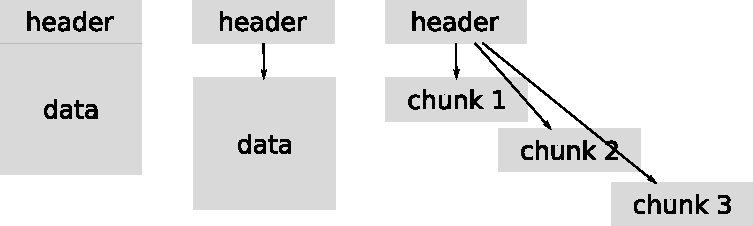
\includegraphics[width=\textwidth]{data_layout.pdf}
%caption{The three data layouts in \textit{DataSet}}
%\label{fig:datalayout}
%\end{figure}
\begin{figure}[ht!]
\resizebox{\textwidth}{!}{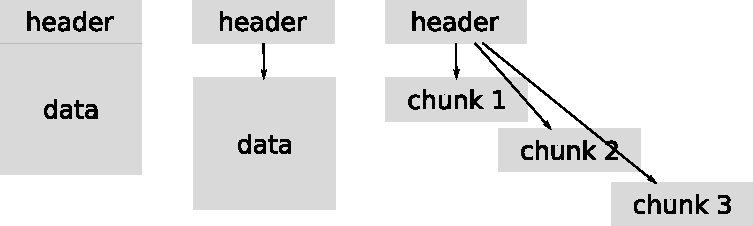
\includegraphics{data_layout.pdf}}
\caption{The three data layouts in \textit{DataSet}}
\label{fig:datalayout}
\end{figure}

If the data is sufficiently small \texttt{H5D\_COMPACT} will be used. In this layout the data address follows right after the header as shown on the left. When the data is bigger but still has a constant size \texttt{H5D\_CONTIGUOUS} is the right layout. This one allows that the address of the data can be arbitrary in memory and is saved in the header. The last layout \texttt{H5D\_CHUNKED} on the right is useful assuming the size of the data is unknown. The data will be divided continuously into chunks with constant size where the address will be saved in the header. This means when a chunk is full a new one gets allocated with its address saved into the header. As the perceptive reader can guess the last layout is of most relevance for this project. A simulation generates new data in each time step which in essence is ideal for the size of a chunk because it further allows to label each chunk to its corresponding time step. This will be later used to match data according to its time label.

\section{DataType}
\label{seq:datatype}
The language C++ itself supports data types such as int, double, char etc. but these cannot be used directly in a binary data format.
This is caused by different data representation which are not homogeneous across different operating systems and system architectures. For example the difference between little-endian and big-endian machines. Thus the library has its own definitions which are compatible across platforms which are incorporated into the different classes seen in figure \ref{graph:hierarchy}. It is intuitively clear from their names which classes must be used to describe which data types. For instance for writing floating point numbers the \textit{FloatType} class is used. In this object further changes of characteristics can be done such as changing from default IEEE representation. In this project the \textit{PredType} and \textit{CompType} are of most relevance. The \textit{PredType} is predetermined meaning there is no explicit constructor needed. From this class \textit{NATIVE\_INT} is used to write the respective time labels for the data. The \textit{CompType} class is utilized for writing complex numbers and also this class has to be explicit constructed which will be explained in section \ref{seq:datatypedec}.

\section{DataSpace}
\label{seq:dataspace}
To describe the dimensionality of our data the \textit{DataSpace} class is required. The construction of such a \textit{DataSpace} is straightforward. Firstly the library needs to know the number of dimensions of the desired space. Secondly it has know the number of elements in each dimension. For the second argument an array of \texttt{hsize\_t} is expected instead of \texttt{int} as described in section \ref{seq:internaltypes}. To give the reader an idea the following code depicts the \textit{DataSpace} of a time grid.

\begin{lstlisting}
int rank = 1;
hsize_t size[rank];
size[0]=number_of_timesteps;
DataSpace limited_timespace(rank,size);
\end{lstlisting}
The problem herein lies in the number of time steps which is known only at runtime but the constructor expects it at compiletime. This leads to another approach which is to define a unlimited \textit{DataSpace}. The library allows this if an additional optional argument is added. This argument has to be of the same data type as the second argument and contains the maximum size of each dimension. The library expects that this argument has to be greater or equal than the previous argument otherwise an exception is thrown. For an unlimited space a special state is used namely \texttt{H5S\_UNLIMITED}. The above example code changes to the following if an unlimited space is desired:
\begin{lstlisting}
int rank = 1;
hsize_t size[rank] = {1};
hsize_t maxsize[rank]={H5S_UNLIMITED};
DataSpace unlimited_timespace(rank,size,maxsize);
\end{lstlisting}

\section{PropList}
Most classes require a specific property list at the moment of construction which include additional information. Depending on the object a different property list is required. All these lists have a common base class namely \textit{PropList} as presented in figure \ref{graph:hierarchy}. The possibilities of these property lists excel the scope of this project easily therefore the default value is enough. The default values are shortly described in table \ref{table:default}.

\begin{figure}[ht!]
\centering
\begin{tabular}{|l|l|}
\hline
Default name value&Influence\\
\hline
\texttt{H5P\_FILE\_CREATE}&\textit{H5FILE} creation\\
\texttt{H5P\_FILE\_ACCESS}&\textit{H5FILE} access\\
\texttt{H5P\_DATASET\_CREATE}&\textit{DataSet} creation\\
\texttt{H5P\_DATASET\_XFER}&raw data transfer\\
\texttt{H5P\_MOUNT}&\textit{H5File} mounting\\
\texttt{H5P\_DEFAULT}&base value for all the above\\
\hline
\end{tabular}
\caption{Table of property list default values and their influence}
\label{table:default}
\end{figure}

Noteworthy for this project is only the \textit{DSetCreatePropList} mentioned in section \ref{seq:dataset} which will be explained in the next section \ref{seq:dscpl}.

\subsection{DSetCreatePropList}
\label{seq:dscpl}
From section \ref{seq:dataset} a \textit{DSetCreatePropList} object is demanded for creating a \textit{DataSet}. As the perceptive reader can guess this property list is used to determine the data layout shown in figure \ref{fig:datalayout}. The property list is responsible for setting the layout to \texttt{H5D\_COMPACT}. This is important because only data with this layout can be dynamically extended later on during a simulation. 

\section{Attribute}
Additionally to writing data in binary format it should also incorporate saving corresponding meta data. This can be easily done with \textit{Attributes} which must be attached to an affiliated \textit{Group} or \textit{DataSet}. The allocation of such an \textit{Attribute} is similar to a \textit{DataSet} meaning a \textit{DataType} and \textit{DataSpace} is also demanded. For its property list only the \texttt{H5P\_DEFAULT} is allowed which the library enforces otherwise an exception is thrown.

\chapter{Writer Template}
\section{Link to Eigen library}
As mentioned in background \ref{seq:background} the simulation boils down to propagating the set \{q,p,Q,P,S\} where q and p are $D$ dimensional real-valued vectors, Q and P complex $DxD$ matrices and S the global complex phase. A possible interface to manage these matrices and vectors is the Eigen library. The definition of an Eigen matrix has the following form:
\begin{lstlisting}
Eigen::Matrix<std::complex<double>,row_dim,column_dim> mat;
\end{lstlisting}
Note that this is a class template over three parameters namely type, row-dimension and column-dimension. Therefore the overall implementation will also be a template. In the current version only scalar \textit{Hagedorn} wavepackets are supported thus only one dimension parameter $D$ is utilized but the framework can still easily be extended in further works. As discussed in section \ref{seq:datatype} normal types are not writable hence the type is defined through the library. This declared type is not necessarily the same as the template argument from Eigen but is still similar enough to permit basic transformation functions.

\section{DataType Declaration}
\label{seq:datatypedec}
In this context simulation means manipulating complex numbers. To build a \textit{DataType} the library needs access to its members thus the standard \texttt{complex} class cannot be utilized. Therefore a \texttt{struct} is most suitable for defining the fundamental structure since all its members are by default public accessible. Hence the declaration of complex numbers looks like this:
\begin{lstlisting}
struct ctype
{
  double real;
  double imag;
} instance_of_ctype;
\end{lstlisting}
This can now be used by the library to create the corresponding \textit{DataType} which in this case the \textit{CompType} is most suitable because \texttt{ctype} is a composition of simple data types. To be compatible with python the same labels for its members has to be used which result in the following code:
\begin{lstlisting}
CompType nctp_(sizeof(instance_of_ctype));
nctp_.insertMember("r",HOFFSET(ctype,real), PredType::NATIVE_DOUBLE);
nctp_.insertMember("i",HOFFSET(ctype,imag), PredType::NATIVE_DOUBLE);
\end{lstlisting}
Worth noting is that the constructor of \textit{CompType} relies on the \texttt{sizeof} operator which tells how many bytes for an instance of this type is needed. The string labels "r" and "i" are utilized for the real respective the imaginary part of a complex number. \texttt{HOFFSET} is a simple function which returns at which position counted in bytes the second argument is located in the first argument. In this simple case because one double is saved in $8$ Bytes \texttt{real} is at position "0" and \texttt{imag} is at position "8". Finally the last argument is the type inserted at this position. Since already discussed in section \ref{seq:datatype} \texttt{double} cannot be used directly but the library provides these definitions through the \textit{PredType} class. The members of \textit{PredType} are constant and are fixed through the C++ language itself.\\

\section{Constructor}
Since the data type declaration has only to be initialized once it is suitable to pack it into the constructor of this writer template. The constructor only expects one string argument namely the filename. Therefore the the constructor can be written accordingly:
\begin{lstlisting}
template<int D>
...
//ctor
hdf5writer(std::string name):filename_(name), nctp_(sizeof(instanceof)),file_(filename_,H5F_ACC_TRUNC)
{
	nctp_.insertMember("r",HOFFSET(ctype,real), PredType::NATIVE_DOUBLE);
	nctp_.insertMember("i",HOFFSET(ctype,imag), PredType::NATIVE_DOUBLE);
}
\end{lstlisting}
Observe that there are two implicit constructor calls after instantiation of the filename. For the former refer to section \ref{seq:datatypedec} for the latter to section \ref{seq:h5file}.

\section{Write options}
To enable customization about what and when something is written an additional layer was inserted. This was done with functions which set the desired configuration. In the current implementation there are three choices to make. By default writing \textit{Hagedorn} wavepackets is enabled and writing norm and energies are disabled with a boolean. As already mentioned in section \ref{seq:dataset} for each chunk written also a time label is attached. This was achieved by writing for each important \textit{DataSet} an additional \textit{DataSet} at the same level with the same length where each entry is an \texttt{int} symbolizing the number of time steps passed since the beginning of the simulation. These are shown in figure \ref{graph:file} where "timegrid" was used in its name. The corresponding customization thereof is to set the difference between two consecutive entries. More precisely it is the choice if a \textit{DataSet} should be written in each time step($d=1$) or every second time step($d=2$) etc. The supported functions are listed subsequently:
\begin{lstlisting}
set_write_packet(true|false);
set_write_norm(true|false);
set_write_energies(true|false);
set_timestep_packet(1|2|3|...);
set_timestep_norm(1|2|3|...);
set_timestep_energies(1|2|3|...);
set_timestep_ekin(1|2|3|...);
set_timestep_epot(1|2|3|...);
\end{lstlisting}

\section{DataSet paths}
The structure in figure \ref{graph:file} is fixed in the implementation as it is analogous to the python generated data. Furthermore the names of all \textit{Groups} and \textit{DataSets} are also already determined. The data test is build on these as well. This can be problematic once a change happens in the python or C++ implementation where the structure is affected. Luckily the library throws an invalid path exception if such a change occurs where the paths are no longer valid. Future work could include to make data test path independent for \textit{DataSets}.

\section{Prestructure}
\label{seq:prestructure}
This function is a bundle of steps which either have to be done prior or are constant during the writing process. The function definition is shown subsequently:
\begin{lstlisting}
template<class MultiIndex>
prestructuring(ScalarHaWp<D,MultiIndex> packet,double dt);
\end{lstlisting}
The dimension $D$ and the class \texttt{MultiIndex} are prerequisite for constructing a scalar \textit{Hagedorn} wavepacket and is detailed explained in the thesis of Michaja B\"osch \cite{bt_michajab}. A scalar \textit{Hagedorn} wavepacket includes a matrix of coefficients and the set \{q,p,Q,P,S\}. The coefficient dimension is dependent on $D$ and \texttt{MultiIndex} therefore the number of coefficients is calculated and stored first in this function. Next the \textit{Groups} of figure \ref{graph:file} is set. Additionally some \textit{Attributes} are attached to the root group such as the time step $dt$. As discussed in section \ref{seq:dataset} each \textit{DataSet} has to be chunked according to a time step. Hence this chunk dimension is set in the next step for all \textit{DataSets} specified in the write options. E.g. for a packet the chunk-dimension for the coefficients, q, p, Q, P, and S have to be set into a instance of \textit{DSetCreatPropList} individually. 
For instance a chunk-dimension is declared in the following form:
\begin{lstlisting}
hsize_t chunk[3] = {1,2,2};//{time_dim,row_dim,column_dim}
\end{lstlisting}
Before it is possible to allocate all \textit{DataSets} according to figure \ref{graph:file} also individual \textit{DataSpaces} have to be declared. Luckily it is possible to reuse all chunk-arrays as arguments for their own \textit{DataSpace} with the additional array argument according to section \ref{seq:dataspace}. Now all building blocks are ready to allocate in the next step all \textit{DataSets}. It can be observed that there is a source and destination \textit{DataSpace} with a selection in each time step. The \textit{DataSpace} is the space of possible positions where data can be written to whereas the a hyperslab is used for the actual selection within the space. The destination \textit{DataSpace} grows over time within the file and thus is not constant. Different from the destination, the source \textit{DataSpace} and its selection is constant and therefore can be fixed in this step for the whole simulation. The workings of a hyperslab as selection is explained in the next section \ref{seq:selection}.

\section{Selection}
\label{seq:selection}
As already mentioned in the previous section \ref{seq:prestructure} a selection within a \textit{DataSpace} is represented with a hyperslab. A hyperslab consists of four arrays namely:
\begin{lstlisting}
hsize_t start[3] = {time_label,1,1};
hsize_t count[3] = {time_label,3,2};
hsize_t block[3] = {time_label,1,1};
hsize_t stride[3] = {time_label,2,2};
\end{lstlisting}
Notice that the first dimension is always reserved for the time dimension. The implementation has an internal index for storing the current simulation step which is used as the label. Thus only the index for the next time step has to be incremented without altering the code for the selection. The following figure \ref{fig:hyperslab} illustrates why four arrays are required to represent a hyperslab.

\begin{figure}[ht!]
\centering
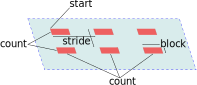
\includegraphics[scale=1.8]{selection.pdf}
\caption{hyper-slab illustration}
\label{fig:hyperslab}
\end{figure}
%TODO explaining figure

The selection is done by the \textit{DataSpace} itself whereas the \texttt{H5S\_SELECT\_SET} argument is recommended to overwrite the old selection.
\begin{lstlisting}
dataspacename.selectHyperslab(H5S_SELECT_SET, count, start, stride, block);
\end{lstlisting}
In case that a continuous block of data is written the last two arguments can be omitted.
\begin{lstlisting}
dataspacename.selectHyperslab(H5S_SELECT_SET, count, start);
\end{lstlisting}


\section{Transformation}
As previously discussed to write data we use our own created data type \textit{nctp}. To write a buffer we need now a pointer of \texttt{ctype}. As such our transformation functions take an \texttt{Eigen::Matrix} with arbitrary template arguments and copies the raw data into a \texttt{std::vector<ctype>} reference. An important implementation detail for data management is the usage of \texttt{std::vector} because the operation system assumes the allocation and deallocation of \texttt{std} objects. Thus our code is much safer in respect to data leaks and data corruption. The \textit{Eigen} library self-manages its matrix objects. To extract \texttt{ctype} pointer from the \texttt{std::vector} object is simple by using the \texttt{.data()} function call.

\section{Writing} 
The writing function call from the HDF library has the following form:
\begin{lstlisting}
datasetname.write(void* src,DataType type,DataSpace srcspace,DataSpace dstspace);
\end{lstlisting}
We already have all tools available to use this function. The \texttt{src} is delivered from the transformation section, \texttt{type} from the declaration section and \texttt{srcspace}, \texttt{dstspace} from the prestucturing sectoin or selection section respectively.

\section{Extension}
For extending a \textit{DataSet} we need the new dimension in a \texttt{hsize\_t} array which is used as the extension. Note here that only chunked \textit{DataSets} are possible to extend with the following call:
\begin{lstlisting}
datasetname.extend(hsize_t extension);
\end{lstlisting}
Also note this function call can also be used to reduce the dimension if the used array \texttt{extension} is smaller then the existing \textit{DataSet}. To know the current position of the data an \texttt{int index} is used for every existing \textit{DataSet}. This index is also used in setting the dimension of the \texttt{hsize\_t extension} array.

\section{Update}
After the extension of a \textit{DataSet} the library doesn't automatically also update the corresponding \textit{DataSpace} which was used in the selection section. As such this is done in this update section. Also the corresponding \texttt{index} to the \textit{DataSet} is incremented in this step. The library provides an easy way to use the extended \textit{DataSet} to set the new \textit{DataSpace} namely:
\begin{lstlisting}
dataspacename = datasetname.getSpace();
\end{lstlisting}
which is done for every existing \textit{DataSet} in the file.
\section{Poststructure}
After the last time step of the simulation we have to finalize our \textit{DataSet} and structures used. This is done in this section. From our implementation we know that also in the last time step we did extend the \textit{DataSet}. As such the last extension will be reversed. Afterwards every structure from the library has to be freed from memory. The system does this automatically for all structures allocated on the stack. For structures which are on the heap because they were allocated with the \texttt{new} operator we have to free them ourselves. This step can be cumbersome because mostly we don't know anymore which object has internally somewhere a reference to it and therefore it is unsafe data management. The implementation avoids this problem by using the \texttt{new} operator to allocate \texttt{std::shared\_ptr} objects which will be managed by the standard library the same as the \texttt{std::vector}. As such the data management is primarily done by the system and not by the implementation.
\section{Inner workings in a picture}
The following figure \ref{fig:illustration} shows the lifetime of a \textit{DataSet} in this implementation. The start signalizes the use of the constructor to allocate the object.
\begin{figure}[ht!]
\resizebox{\textwidth}{!}{
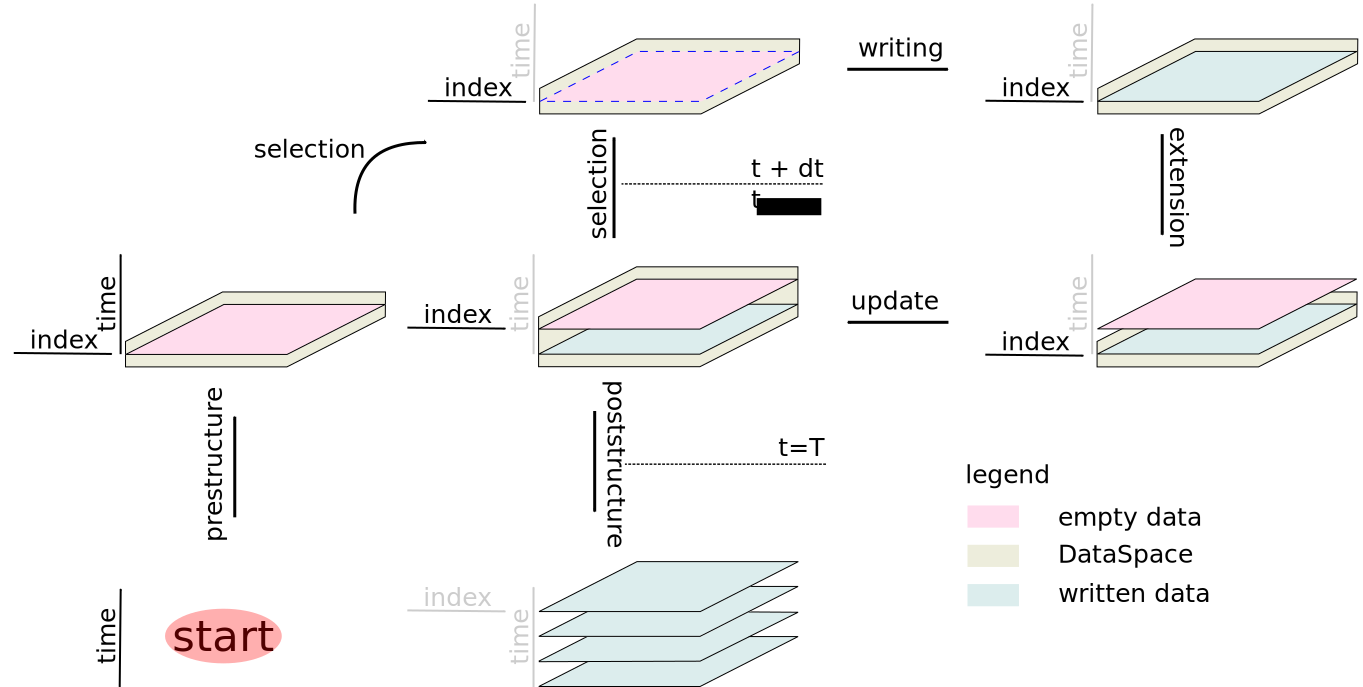
\includegraphics[scale=1.0]{writing_dataset.pdf}
}
\caption{Illustration of inner workings for a \textit{DataSet} in the simulation}
\label{fig:illustration}
\end{figure}

\section{Usage in a simulation main file}
Note that this implementation is only able to write scalar \textit{Hagedorn} wave packets with the normal \textit{Hagedorn} parameter set for the moment. Further work includes to either extend this HDF5 writer template with matching functions for more complicated \textit{Hagedorn} wave packets or to generalize the template on these packets. In the simulation the packet and its parameter set is constructed in the following form:
\begin{lstlisting}
...
wavepackets::HaWpParamSet<D> param_set(q,p,Q,P,S);
...
wavepackets::ScalarHaWp<D,MultiIndex> packet;
...
\end{lstlisting}
%
%TODO reference zu Michja wie ScalarHawp implementiert isch
%
Hence our HDF5 writer template is constructed and used in the following way:
\begin{lstlisting}
... //setting simulation variables, options etc.

//constructor of this template implementation
io::hdf5writer<D> writer("simulation_filename.hdf5");

//optional setup write options
bool write_packet,write_energy,write_norm;
write_packet=true;//default value
write_energy=false;//default value
write_norm=false;//default value
writer.set_write_energy(write_packet);
writer.set_write_norm(write_energy);
writer.set_write_packet(write_norm);
int packet_stepsize,energy_stepsize,norm_stepsize;
packet_stepsize=1;//default value writing every time step
energy_stepsize=1;//default value writing every time step
norm_stepsize=1;//default value writing every time step
writer.set_timestep_packet(packet_stepsize)
writer.set_timestep_energy(energy_stepsize)
writer.set_timestep_norm(norm_stepsize)

//optional setup write paths
std::string datablockstring,wavepacktstring,packetgroupstring;
std::string coefficientgroupstring,energiesgroupstring;
std::string normsgroupstring,observablesgroupstring;
//default paths see figure @\ref{graph:file}@
datablockstring="/datablock_0";
wavepacktstring="/wavepacket";
packetgroupstring="/Pi";
coefficientgroupstring="/coefficients"
energiesgroupstring="/energies"
normsgroupstring="/norm";
observablesgroupstring="/observables";
writer.set_datablockstring(datablockstring);
writer.set_wavepacketstring(wavepacktstring);
writer.set_packetgroupstring(packetgroupstring);
writer.set_coefficientgroupstring(coefficientgroupstring);
writer.set_energiesgroupstring(energiesgroupstring);
writer.set_normsgroupstring(normsgroupstring);
writer.set_observablesgroupstring(observablesgroupstring);

//prestructuring step
writer.prestructuring<MultiIndex>(packet,dt);

//simulation loop body
for(real_t t = 0; t < T; t += dt)
{
	real_t ekin=observables::kinetic_energy<D,MultiIndex>(packet);
	real_t epot=observables::potential_energy<ScalarMatrixPotential<D>,D,MultiIndex,TQR>(packet,V);
	writer.store_packet(packet); //function call for storing packet in file
	writer.store_energies(epot,ekin); //function call for storing energies in file
	writer.store_norm(packet); //function call for storing norm in file	
}

//finalization with postructure
writer.poststructuring();
\end{lstlisting}
Remember that only the constructor, prestructuring and poststructuring are always mandatory independent of the simulation. Also note that if write option of norm and/or energies is set to true but the \texttt{.store\_...} function call is missing that an error message will be printed without aborting the simulation. 

\chapter{Data Test}

\section{Introduction to GoogleTest}
There are two main ways to test objects with this framework. For the interested reader a more detailed documentation can be found in the git repository \cite{googletestdoc} where the Primer.md and AdvancedGuide.md examples are strongly suggested. Of importance is to define a test class for reusing certain objects for all tests. These objects in this case are the two \textit{H5Files}, the \textit{DataType} used in the writing process and the \textit{Attributes} saved in the root group of the two files. One of these \textit{Attributes} is the used time step $\Delta t$ in the simulation which will be needed later for a data matching.

\section{The Main C++ File}
The data test main file is of the following structure:
\begin{lstlisting}
#include "gtest/gtest.h"
int global_argc;
char** global_argv;
...

class TestHDF : public ::testing::Test
{
	protected:
	TestHDF();
	virtual ~TestHDF();
	void SetUp();
	void TearDown();
	void time_matching(...);
	
	struct ctype{...};
	H5File cppfile;
	H5File pyfile;
	CompType nctp;
	double dt_cpp;
	double dt_py;
	...
};

TEST_F(TestHDF,Testpacket)
{...}
TEST_F(TestHDF,Testenergies)
{...}
TEST_F(TestHDF,Testnorm)
{...}

int main(int argc,char* argv[])
{
	global_argc=argc;
	global_argv=argv;
	::testing::InitGoogleTest(&argc,argv);
	return RUN_ALL_TESTS();
}
\end{lstlisting}

%TODO overwork
Note that \texttt{TEST\_F} are test fissures which uses the same class object \texttt{TestHDF}. In the constructor the filenames are loaded in the \texttt{H5File} objects and the \textit{CompType} is also set the same as in section \textit{DataType} declaration. For each test fissure the \texttt{SetUp} function is used for further construction and at the end cleaned with \texttt{TearDown} function. To transfer the filenames, which are delivered over the command line arguments, global variables are used. In the respective test fissures the data of the two files will be compared relative to an absolute tolerance error. Hereby it has to be known which time points can be compared to in a general case. This is done with the \texttt{time\_matching} function which saves the matching time points in vector, where every entry are two indices, and as arguments two paths, represented as strings with the same form as in group section, to the respective time grid \textit{DataSet}.

\chapter{Conclusion}



\appendix

\chapter{Appendix}

\section{Code of 2D harmonic oscillator}
\begin{lstlisting}
#include <iostream>
#include <fstream>

#include "waveblocks/types.hpp"
#include "waveblocks/wavepackets/shapes/tiny_multi_index.hpp"
#include "waveblocks/potentials/potentials.hpp"
#include "waveblocks/potentials/bases.hpp"
#include "waveblocks/wavepackets/hawp_paramset.hpp"
#include "waveblocks/wavepackets/hawp_commons.hpp"
#include "waveblocks/wavepackets/shapes/shape_enumerator.hpp"
#include "waveblocks/wavepackets/shapes/shape_hypercubic.hpp"
#include "waveblocks/innerproducts/gauss_hermite_qr.hpp"
#include "waveblocks/innerproducts/tensor_product_qr.hpp"
#include "waveblocks/propagators/Hagedorn.hpp"
#include "waveblocks/observables/energy.hpp"
#include "waveblocks/io/hdf5writer.hpp"


using namespace waveblocks;

int main() {
    const int N = 1;
    const int D = 2;
    const int K = 4;

    const real_t sigma_x = 0.5;
    const real_t sigma_y = 0.5;

    const real_t tol = 1e-14;

    const real_t T = 12;
    const real_t dt = 0.01;

    const real_t eps = 0.1;

    using MultiIndex = wavepackets::shapes::TinyMultiIndex<unsigned long, D>;

    // The parameter set of the initial wavepacket
    CMatrix<D,D> Q = CMatrix<D,D>::Identity();
    CMatrix<D,D> P = complex_t(0,1) * CMatrix<D,D>::Identity();
    RVector<D> q = {-3.0, 0.0};
    RVector<D> p = { 0.0, 0.5};
    complex_t S = 0.0;
    wavepackets::HaWpParamSet<D> param_set(q,p,Q,P,S);

    // Basis shape
    wavepackets::shapes::ShapeEnumerator<D, MultiIndex> enumerator;
    wavepackets::shapes::ShapeEnum<D, MultiIndex> shape_enum = enumerator.generate(wavepackets::shapes::HyperCubicShape<D>(K));

    // Gaussian Wavepacket phi_00 with c_00 = 1
    Coefficients coeffs = Coefficients::Zero(std::pow(K, D), 1);
    coeffs[0] = 1.0;
    Coefficients coefforig = Coefficients(coeffs);

    // Assemble packet
    wavepackets::ScalarHaWp<D,MultiIndex> packet;
    packet.eps() = eps;
    packet.parameters() = param_set;
    packet.shape() = std::make_shared<wavepackets::shapes::ShapeEnum<D,MultiIndex>>(shape_enum);
    packet.coefficients() = coeffs;

    // Defining the potential
    typename CanonicalBasis<N,D>::potential_type potential =
        [sigma_x,sigma_y](CVector<D> x) {
        return 0.5*(sigma_x*x[0]*x[0] + sigma_y*x[1]*x[1]).real();
    };
    typename ScalarLeadingLevel<D>::potential_type leading_level = potential;
    typename ScalarLeadingLevel<D>::jacobian_type leading_jac =
        [sigma_x,sigma_y](CVector<D> x) {
        return CVector<D>{sigma_x*x[0], sigma_y*x[1]};
    };
    typename ScalarLeadingLevel<D>::hessian_type leading_hess =
        [sigma_x,sigma_y](CVector<D> /*x*/) {
        CMatrix<D,D> res;
        res(0,0) = sigma_x;
        res(1,1) = sigma_y;
        return res;
    };

    ScalarMatrixPotential<D> V(potential,leading_level,leading_jac,leading_hess);

    // Quadrature rules
    using TQR = innerproducts::TensorProductQR<innerproducts::GaussHermiteQR<K+4>,
                                               innerproducts::GaussHermiteQR<K+4>>;

    // Defining the propagator
    propagators::Hagedorn<N,D,MultiIndex, TQR> propagator;

    io::hdf5writer<D> writer("harmonic_2D_cpp.hdf5");
    writer.set_write_energies(true);
    writer.set_write_norm(true);
    writer.prestructuring<MultiIndex>(packet,dt);

    // Time loop(propagation)
    for (real_t t = 0; t < T; t += dt) {
    	real_t ekin = observables::kinetic_energy<D,MultiIndex>(packet);
        real_t epot = observables::potential_energy<ScalarMatrixPotential<D>,D,MultiIndex,TQR>(packet,V);

        writer.store_packet(packet);
        writer.store_energies(epot,ekin);
        writer.store_norm(packet);
    	
        // Propagate
        propagator.propagate(packet,dt,V);

        // Assure constant coefficients
        auto diff = (packet.coefficients() - coefforig).array().abs();
        auto norm = diff.matrix().template lpNorm<Eigen::Infinity>();
        bool flag = norm > tol ? false : true;
        assert(flag);
    }
    writer.poststructuring();
}
\end{lstlisting}


\backmatter

\bibliographystyle{plain}
\bibliography{refs,own,wp,references}

%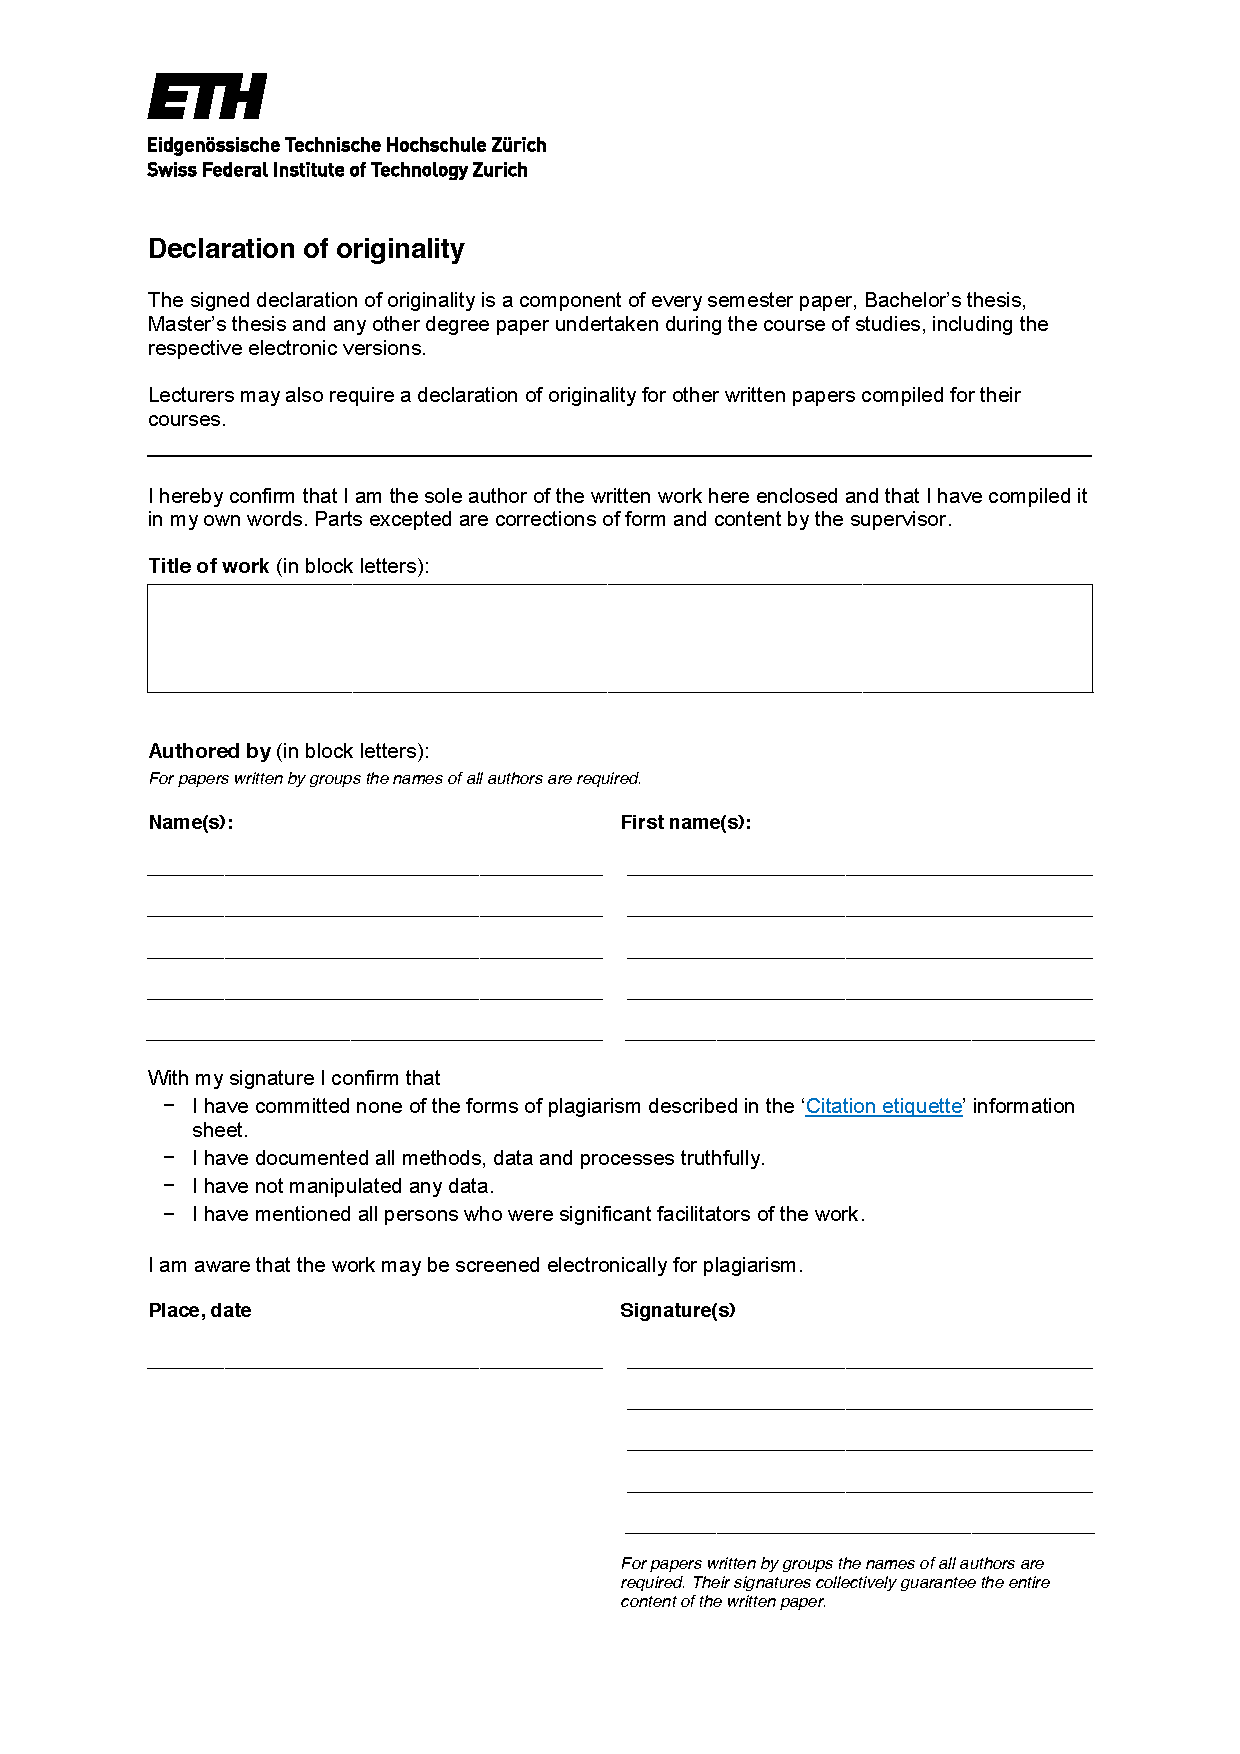
\includepdf[pages={-}]{declaration-originality.pdf}

\end{document}
